\chapter{Výsledky}\label{chap:results}

V tejto kapitole uvedieme dosiahnuté výsledky namerané spôsobom popísaným v predošlej kapitole \ref{chap:proposal_and_implementation}. Obsahuje záznam o zmene presnosti trojfázového trénovania na datasete NYUHands. Ďalej uvedieme ako sa menila presnosť počas trénovania na našom datasete.% a ukážeme úspešné aj neúspešné prípady predikcie kĺbov na obrázkoch. Porovnáme náš systém s niekoľkými podobnými prácami.

Pre všetky vyhodnocovania sme vytvorili dva grafy v dvoch stĺpcoch, kde graf na ľavej strane zobrazuje celkovú presnosť, teda priemernú hodnotu z presností všetkých kĺbov. Červenou je znázornená presnosť pre tie kĺby, ktorých predikované súradnice boli vzdialené od očakávaných súradníc do 2mm a modrou do 5mm. Uvádzané výsledky sú v tolerancii 5mm. Graf na pravej strane zobrazuje presnosť predikcie pre jednotlivé kĺby. Na tomto grafe sme použili označenie k\_prst a znamená, že dané hodnoty prislúchajú končeku daného prsta.

Náš systém predikuje 2D súradnice a preto sme vyhodnocovali predikciu pre RGB obrázky a súradnice v 2D. Na vyhodnocovanie prvej časti trénovania na NYUHands datasete sme používali obrázky z validačnej množiny.%Vďaka kamere máme RGB obrázky a hĺbkové dáta zarovnané, teda pixlu so súradnicami v RGB obrázku prislúcha hĺbková informácia na rovnakých súradniciach aj v hĺbkovej mape.

V prvej fáze trénovania sme nastavili počítanie chyby pre konček palca. Dosahovaná presnosť pre každú epochu je zobrazená na Obr. \ref{img:50thumbAcc}.  V tejto fáze učenia je teda vidieť zlepšenie predikcie pre konček palca a presnosť predikcie pre ostatné kĺby je blízka nule. Do druhej fázy sme vybrali také nastavenie váh ktoré dosiahlo najvyššiu presnosť podľa predikcie palca. Vrchol bol dosiahnutý v 39. epoche s presnosťou 52,74\%.

\begin{figure}[H]
	\begin{center}
		\makebox[\textwidth]{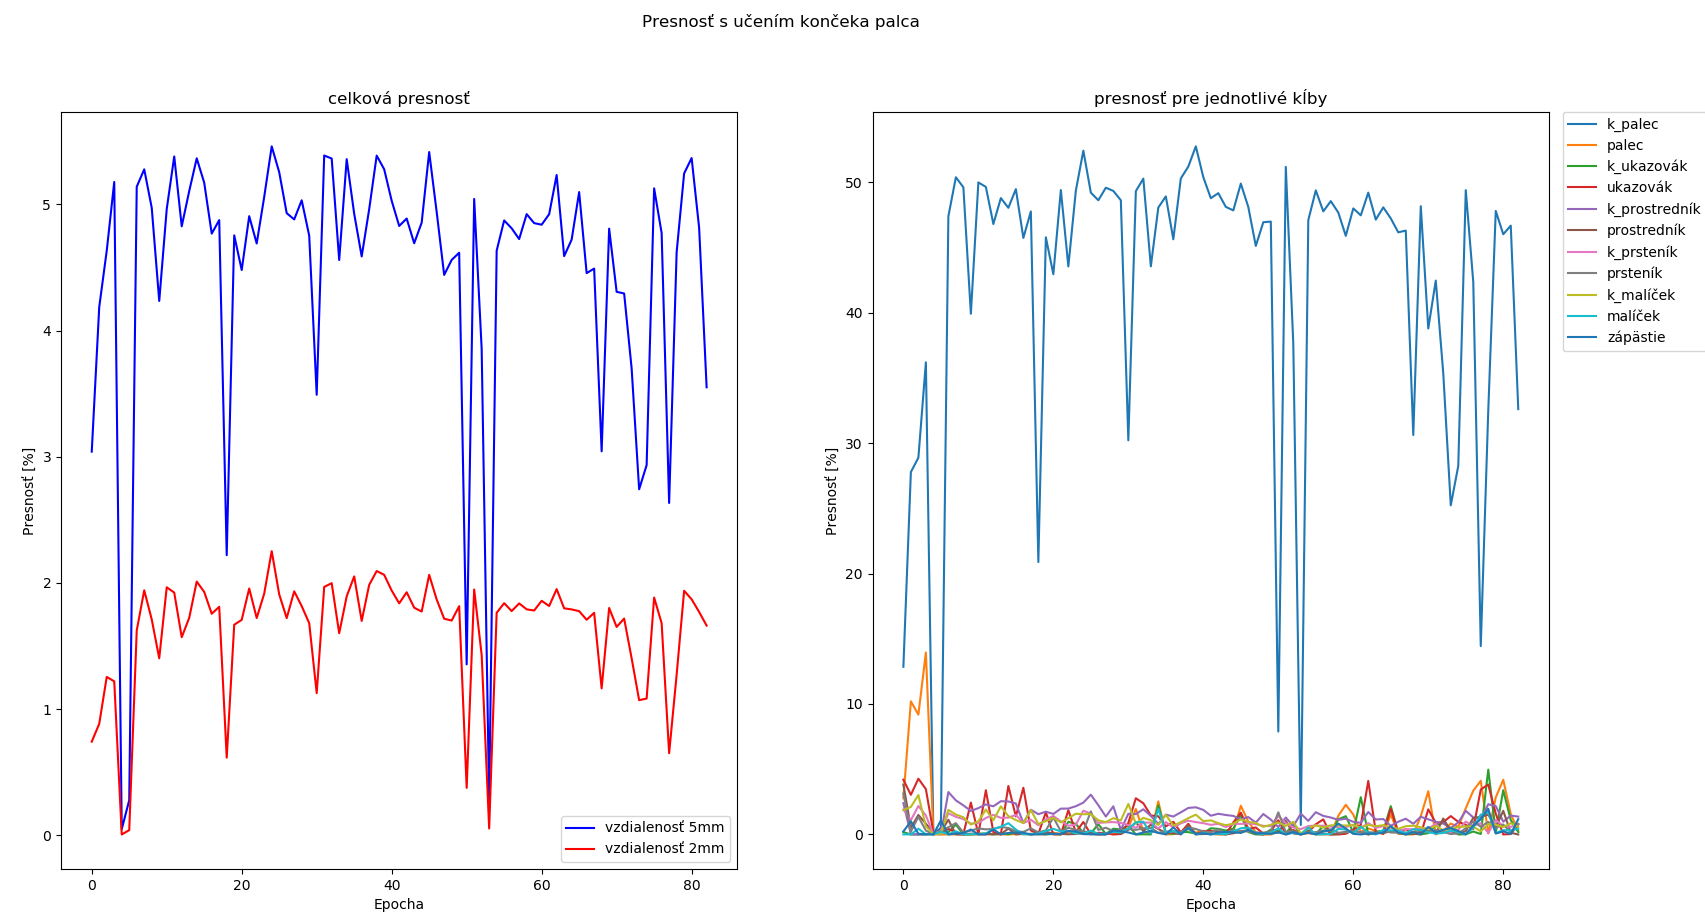
\includegraphics[width=\textwidth]{images/50thumbAcc.png}}
		\caption{Priebeh učenia prvej fázy s počítaním chyby pre konček palca.}
		\label{img:50thumbAcc}
	\end{center}
\end{figure}

Druhá fáza mala nastavené počítanie chyby pre všetky končeky prstov. Priebeh dosahovaných presností je zobrazený na Obr. \ref{img:51fingertipsAcc}. Keďže chceme náš model aj čo najlepšie generalizovať a nie ho iba sústrediť na najlepšie určenie jedného kĺbu, tak sme vybrali najvhodnejšie nastavenie váh podľa najvyššej priemernej presnosti z trénovaných kĺbov. Tá bola dosiahnutá v ôsmej epoche s priemernou presnosťou určenia končekov prstov 56,91\%.

\begin{figure}[H]
	\begin{center}
		\makebox[\textwidth]{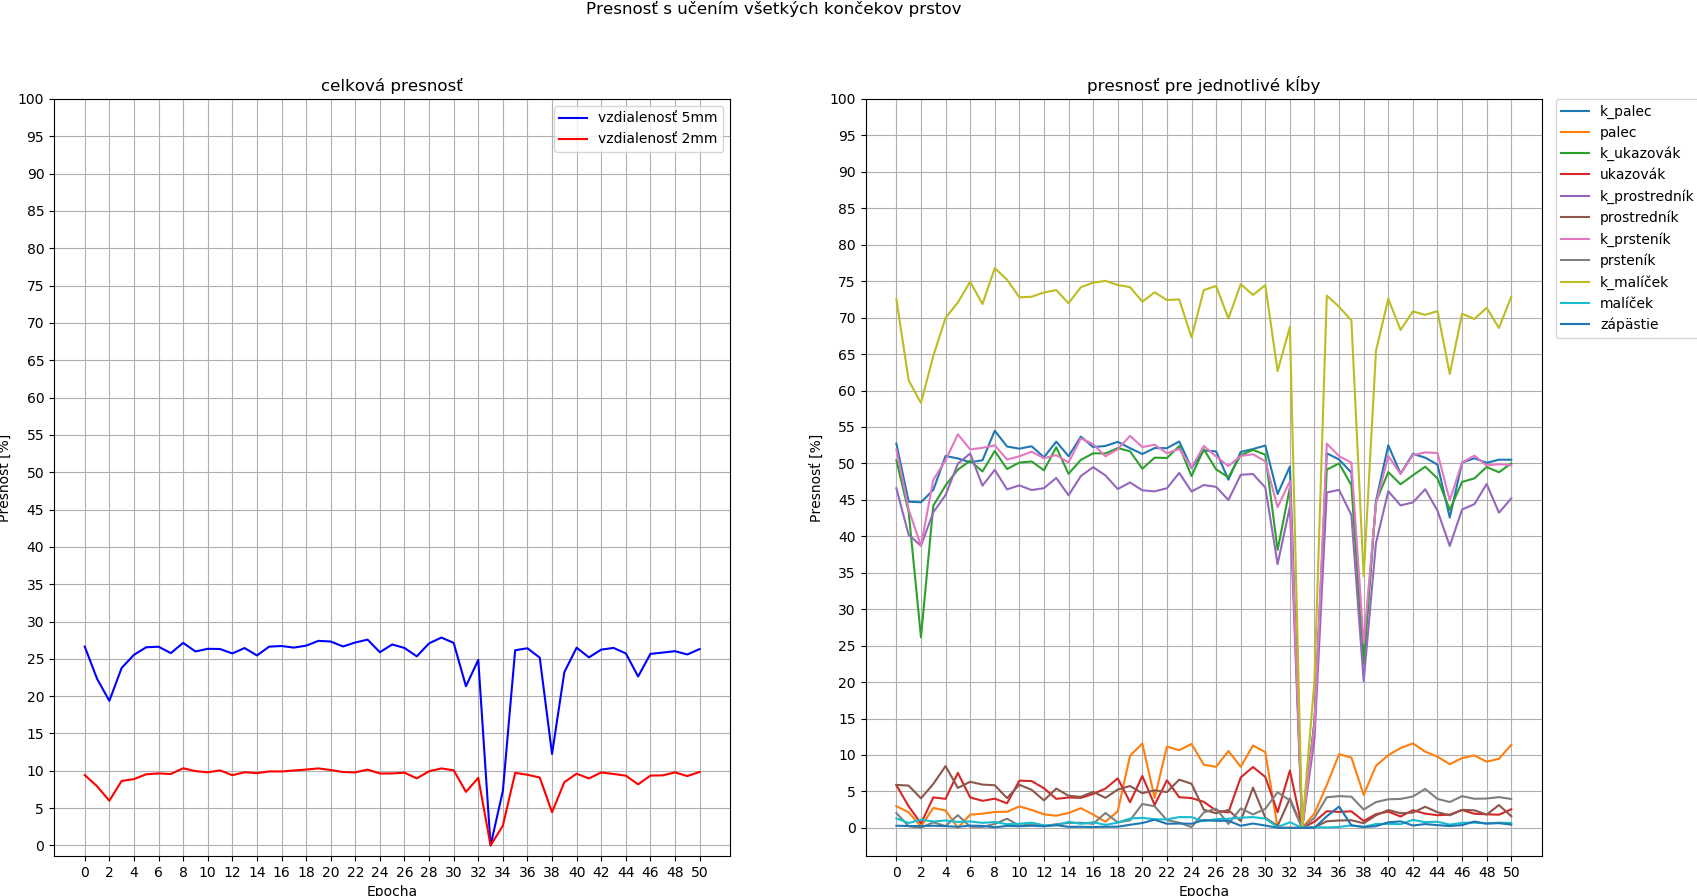
\includegraphics[width=\textwidth]{images/51fingertipsAcc.png}}
		\caption{Priebeh učenia druhej fázy. Počítanie chyby pre končeky prstov.}
		\label{img:51fingertipsAcc}
	\end{center}
\end{figure}

Pre tretiu fázu sme inicializovali váhy z ôsmej epochy predošlého kroku. Vývoj presnosti počas učenia je zobrazený na obr. \ref{img:52jointsAcc}. Celkovú presnosť predikcie na NYUhands náš systém dosiahol 64,48\% v štrnástej epoche.

\begin{figure}[H]
	\begin{center}
		\makebox[\textwidth]{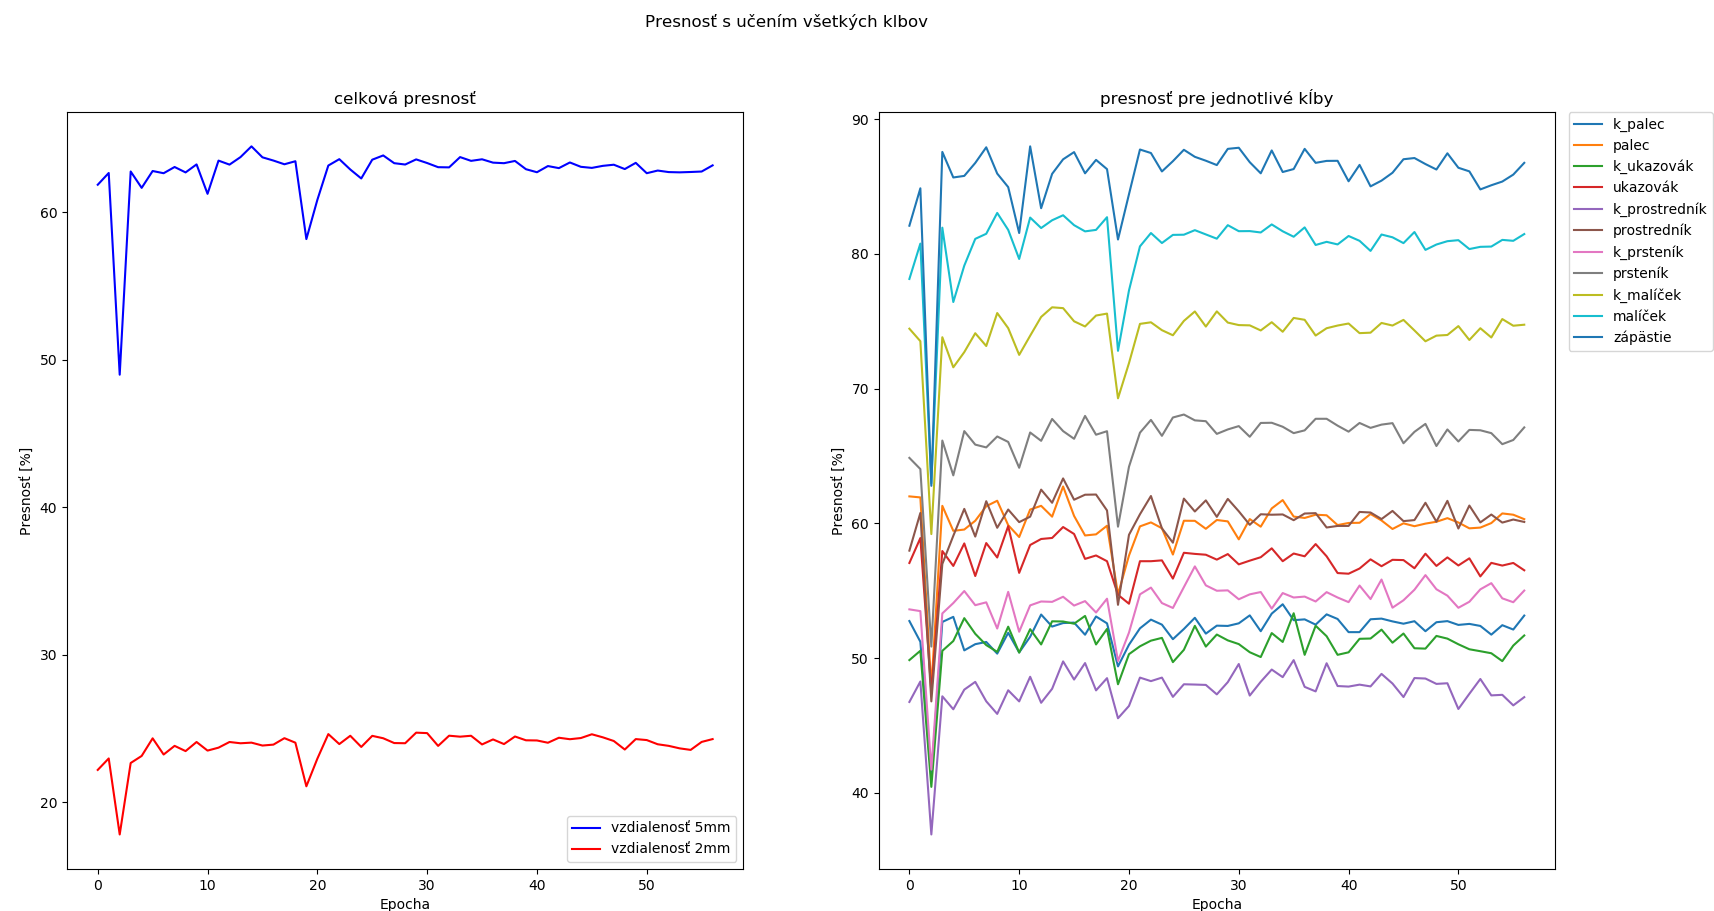
\includegraphics[width=\textwidth]{images/52jointsAcc.png}}
		\caption{Priebeh učenia tretej fázy s počítaním chyby pre všetky kĺlby.}
		\label{img:52jointsAcc}
	\end{center}
\end{figure}

Náš dataset sme dotrénovali na sieti s inicializáciou váh zo 3trn8stej epochy predošlého trénovania. Vývoj presnosti je na obr. \ref{img:53myAcc}. Keďže v ňom máme veľmi málo obrázkov, rýchlo sa sieť naučila predikovať celkom presne súradnice kĺbov. Preto sme pre výber brali do úvahy väčší dôraz na presnosť s odchýlkou 2mm a vybrali sme taký model, ktorý viac kĺbov určil s presnosťou do tejto vzdialenosti. Taký výsledok bol dosiahnutý v 219. epoche s presnosť na 2mm bola úspešnosť 81.81\% a na 5mm 99.54\%.

\begin{figure}[H]
	\begin{center}
		\makebox[\textwidth]{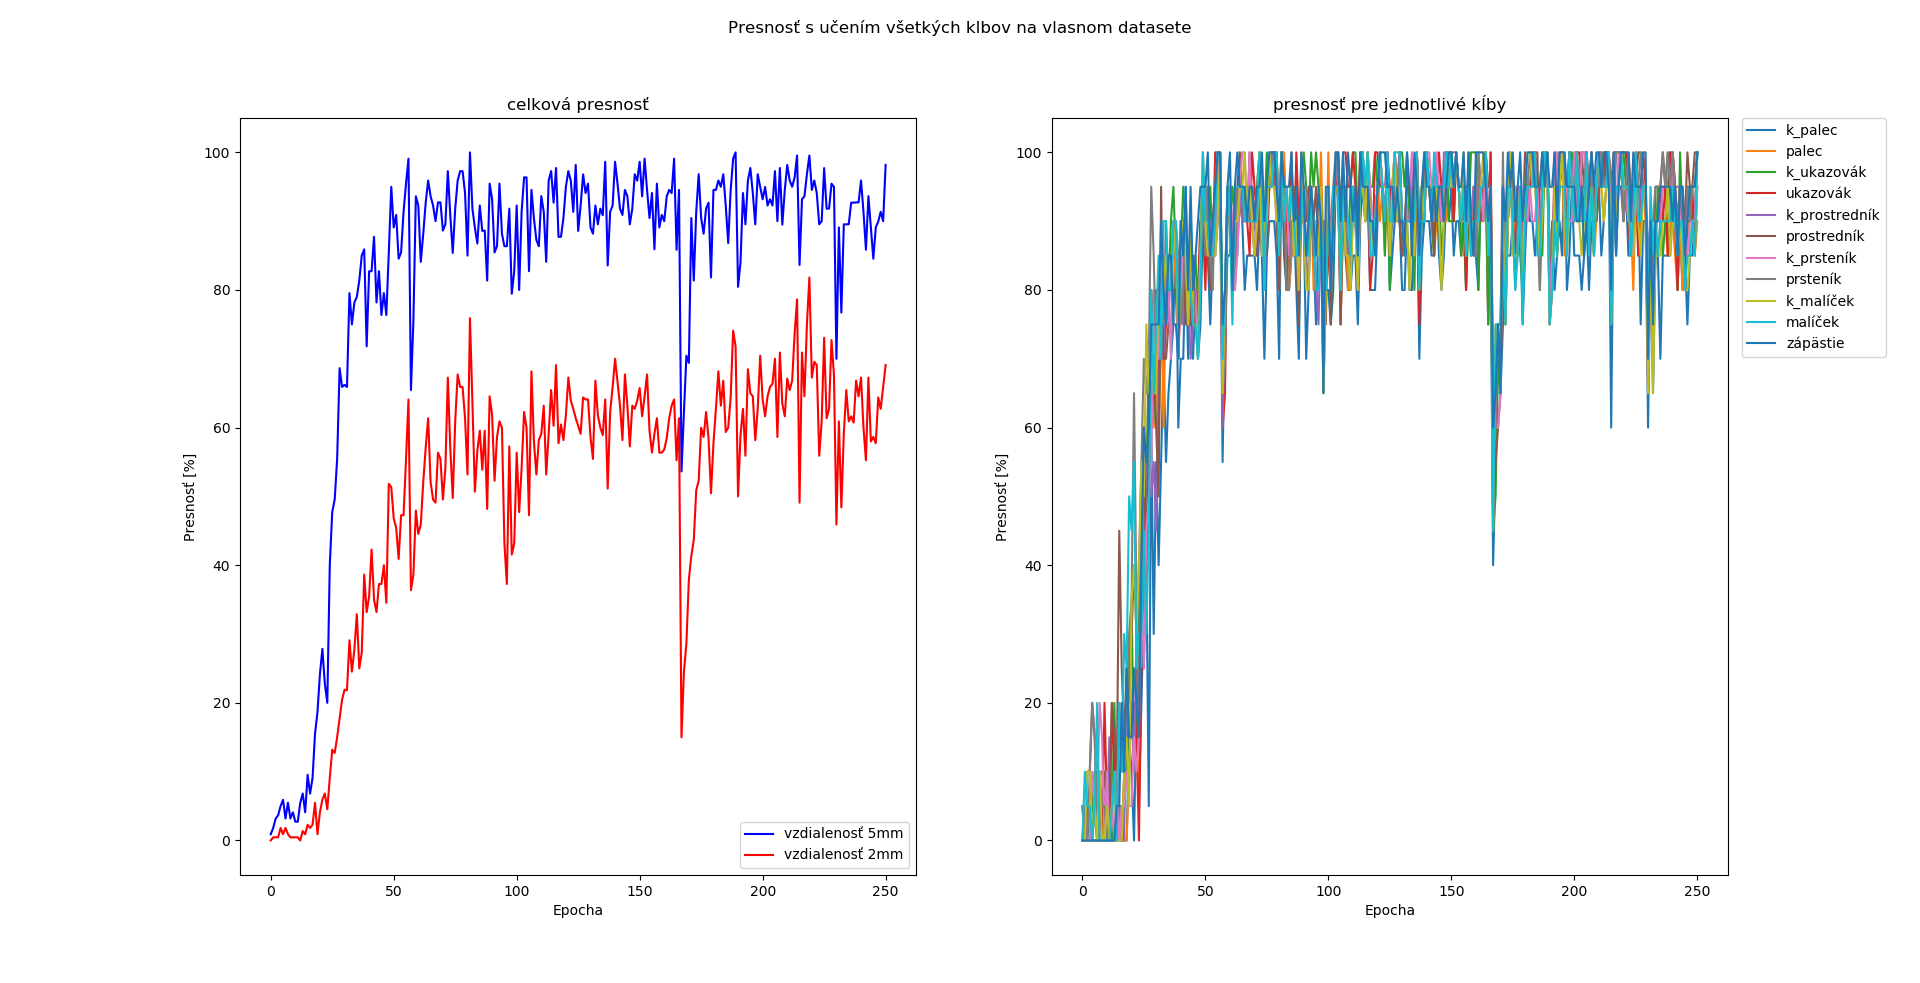
\includegraphics[width=\textwidth]{images/53myAcc.png}}
		\caption{Priebeh učenia predikcie pozície kĺbov na našom datasete.}
		\label{img:53myAcc}
	\end{center}
\end{figure}